\documentclass[tikz,border=10pt]{standalone}
\usepackage{amsmath}
\usepackage{tikz}
\usetikzlibrary{arrows.meta, positioning, angles, quotes, decorations.markings, calc}

\begin{document}

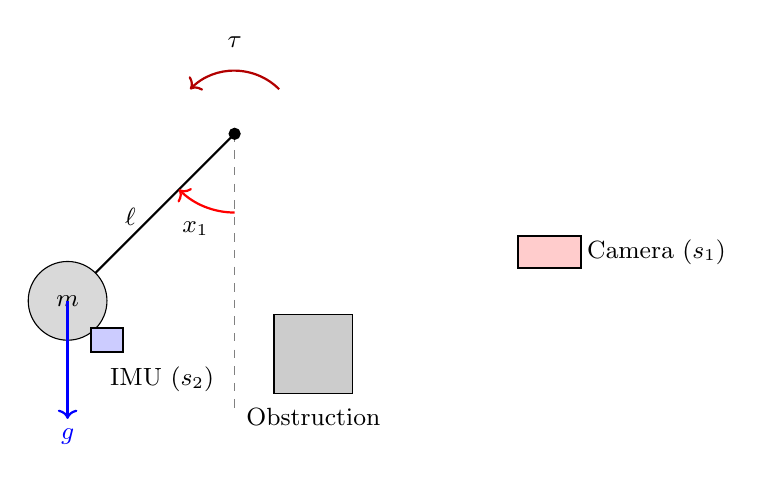
\begin{tikzpicture}[
  mass/.style = {circle, draw, fill=gray!30, minimum size=1cm},
  string/.style = {thick},
  anglemark/.style = {draw, ->, thick, red},
  force/.style = {->, thick, blue},
  arrow/.style = {thick, -{Latex[width=2mm]}},
  torque/.style = {->, thick, red!70!black},  
  sensor/.style = {draw, thick, rectangle, fill=red!20, minimum width=0.8cm, minimum height=0.4cm},
  obstruction/.style = {draw, fill=gray!40, minimum width=1cm, minimum height=1cm},
  every node/.style = {font=\small}
]

% Parameters
\def\L{3}
\def\theta{45} % degrees

% Coordinates
\coordinate (pivot) at (0,0);
\coordinate (bob) at ($(pivot) + (\theta:-\L)$);
\coordinate (equilibrium) at ($(pivot) + (270:\L)$);

% Pendulum and rod
\draw[dashed, gray] (pivot) -- ++(270:\L+0.5); % vertical reference
\draw[string] (pivot) -- (bob);
\node[mass] at (bob) {$m$};
\filldraw[black] (pivot) circle (2pt);

% Angle and state labels
\draw[anglemark] (pivot) ++(270:1) arc[start angle=270, end angle={270 - \theta}, radius=1];
\node at ($(pivot)+({270 - 0.5*\theta}:1.3)$) {$x_1$};


% Gravity
\draw[force] (bob) -- ++(0,-1.5) node[below] {$g$};

% Length label
\path (pivot) -- node[midway, left=2pt] {$\ell$} (bob);

% Torque input
\draw[torque] ([shift=(45:0.8cm)]pivot) arc[start angle=45, end angle=135, radius=0.8];
\node[above=2pt] at ($(pivot)+(90:0.9)$) {$\tau$};

% Sensor 1: Camera + laser beam (from right)
\coordinate (camera) at (4, -1.5);
\node[sensor, rotate=0] at (camera) {};
\node[right=10pt] at (camera) {Camera $(s_1)$};

% Sensor 2: IMU mounted on mass
\node[sensor, minimum width=0.4cm, minimum height=0.3cm, fill=blue!20] at ($(bob)+(0.5,-0.5)$) {};
\node at ($(bob)+(1.2,-1
)$) {IMU $(s_2)$};

% Obstruction (in front of equilibrium position)
\coordinate (obstruction) at ($(pivot) + (270:\L-0.2) + (1,0)$);
\node[obstruction, anchor=center] at (obstruction) {};
\node at ($(obstruction)+(0,-0.8)$) {Obstruction};

\end{tikzpicture}

\end{document}
